\section{Park Details}
\label{parkDetails}

In den Details der einzelnen Parks findet man eine \nameref{map} mit zwei Marker. Ein Marker für die 
Position des Parks und ein anderer f+r die derzeitige Position des Benutzers. Verweigert der 
Benutzer, dass auf seinen Standort zugegriffen werden darf, wird nur ein Marker an der Position des
Parks platziert.

\begin{figure}[H]
    \begin{center}
      \frame{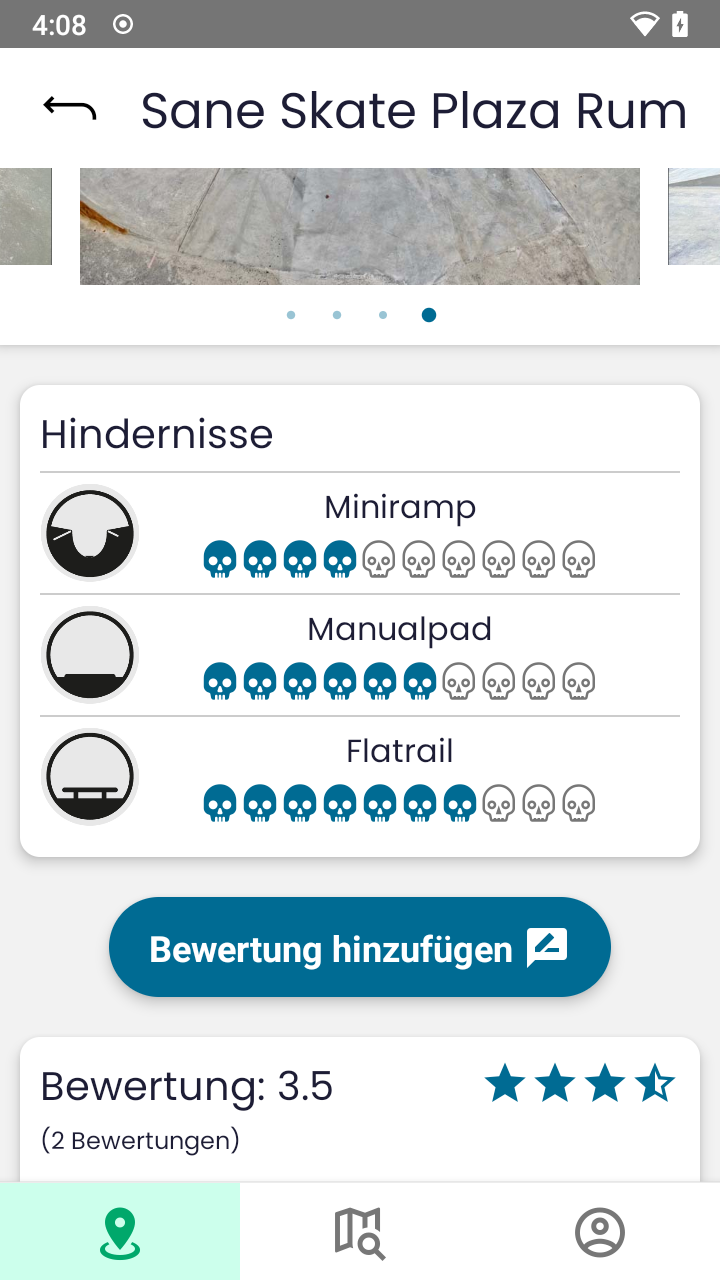
\includegraphics[width=1\textwidth]{Website/Obstacles.png}}
      \caption{Die Startseite}
    \end{center}
\end{figure}

Unterhalb der Map stehen die Hindernisse welche sich in dem Park befinden. Schwebt man mit der Maus 
über eins der Hindernisse wird der Name und die Schwierigkeit des Hindernisses angegeben. Die Daten 
über das Hindernis und über den Park selbst, wird durch einen \textit{useFetch} in Erfahrung 
gebracht. Ist man mit einem Benutzer angemeldet, kann man unter den Hindernissen eine Bewertung 
schreiben.
\pagebreak
\subsection{Bewertungen}

\begin{figure}[H]
  \begin{center}
    \frame{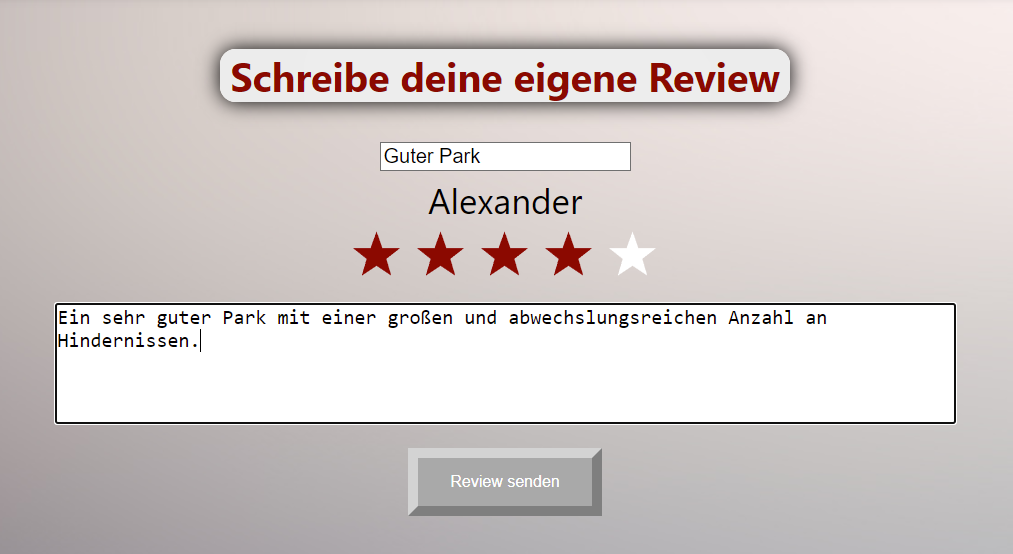
\includegraphics[width=1\textwidth]{Website/Review-Schreiben.png}}
    \caption{Die Startseite}
  \end{center}
\end{figure}

Damit es möglich ist eine Review zu schreiben muss ein Titel angegeben sein. Unter dem Titel steht 
der Benutzername des eingeloggten Users. Mit einem Klick auf den Sternen kann man dem Park eine 
Bewertung von eins bis fünf geben. Diese Sternenbewertung wurde mittels einer externen React 
Komponente names \textbf{React Star Ratings} von \textbf{ekeric13} gemacht. Drückt man auf den 
Senden Knopf wird die Review an den Server gesendet, welcher den dann in die Datenbank speichert. 
Während die Review and den Server gesendet wird, ist der Knopf deaktiviert, damit man bei wiederholten 
Knopfdruck nicht mehrere male eine Review and den Server sendet.

\begin{figure}[H]
  \begin{center}
    \frame{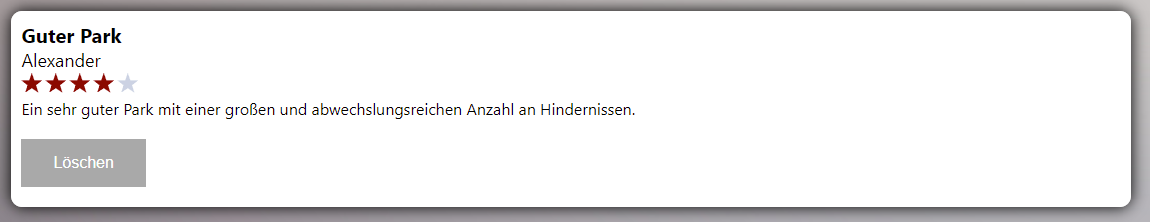
\includegraphics[width=1\textwidth]{Website/Review.png}}
    \caption{Eine geschriebene Bewertung}
  \end{center}
\end{figure}

Unter dem erstellen einer Bewertung kann man alle anderen Bewertungen dieses Parks sehen. Es ist möglich 
seine eigene Bewertung zu löschen. Dies erfolgt ganz einfach über die Überprüfung der BenutzerId mit 
der BenutzerId des Herstellers der Bewertung.